\documentclass[tikz,dvipsnames]{standalone}
\usepackage{amsmath} 
\usepackage{amssymb}
\usepackage{bm}
\usepackage{pgfplots}
\pgfplotsset{compat=1.18}
\usepackage{xstring}


\begin{document}

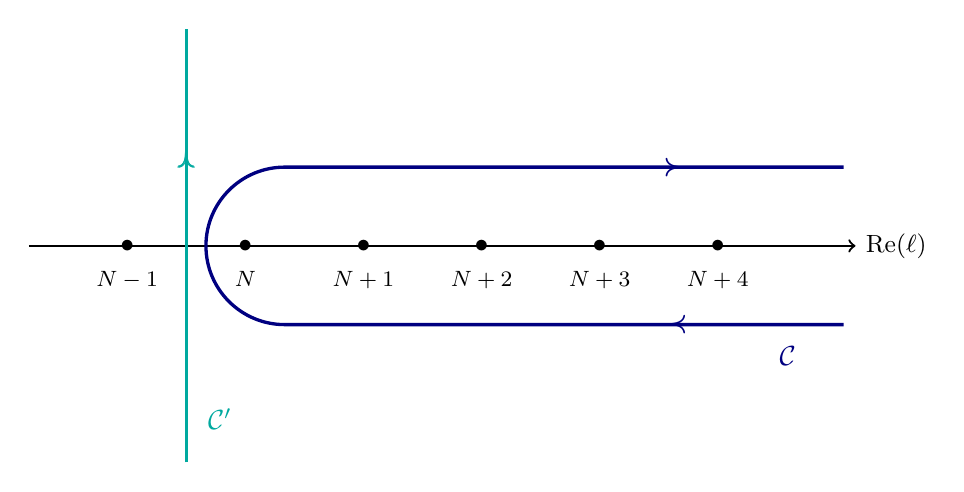
\begin{tikzpicture}
    \draw[->,thick] (-3.5*1.5,0)--(3.5*1.5,0) node[right]{\small{$\operatorname{Re}(\ell)$}};

    \newcommand*\GetListMember[2]{\StrBetween[#2,\number\numexpr#2+1]{,#1,},,\par}
    \newcommand*\lablist{$N-1$,$N$,$N+1$,$N+2$,$N+3$,$N+4$}

    \pgfmathsetmacro\n{6}
     
    \foreach \i in {1,...,\n} {
        \node[label=below:\footnotesize{\GetListMember{\lablist}{\i}}] at (\i*1.5-5.5,0) {$\bullet$};
        }
        
    \draw[very thick,Emerald] (-3.25,-2.75)--(-3.25,2.75) node[pos=0.7,color=Emerald] {$\bm{\curlywedge}$} node[pos=0.1,label=right:$\mathcal{C}'$] {};

    \draw[very thick,NavyBlue](3.4*1.5,1)--node[pos=0.3,color=NavyBlue] {$\bm{\succ}$} (-2,1) arc (-270:-90:1) -- (3.4*1.5,-1) node[pos=0.7,color=NavyBlue] {$\bm{\prec}$} node[pos=0.9,label=below:$\mathcal{C}$]{};

\end{tikzpicture}

\end{document}